\documentclass[handout, aspectratio = 169]{beamer}
%\documentclass[presentation]{beamer}

%https://www.overleaf.com/project/5f638086f8e558000137cf72

\usecolortheme{Imperial}
 
\usepackage[utf8]{inputenc}
\usepackage[UKenglish]{babel}
\usepackage{booktabs}
\usepackage{caption}
\usepackage{subcaption}
\usepackage{graphicx}
\usepackage{amsmath}
\usepackage{amsfonts}
\usepackage{amssymb}
\usepackage{epstopdf}
\usepackage{animate}
\usepackage{fancyvrb}

% complying UK date format, i.e. 1 January 2001
\usepackage{datetime}
\let\dateUKenglish\relax
\newdateformat{dateUKenglish}{\THEDAY~\monthname[\THEMONTH] \THEYEAR}

% Imperial College Logo, not to be changed!
\institute{
\includegraphics[height=0.7cm]{Imperial_1_Pantone_solid.eps}}



% -----------------------------------------------------------------------------

\setbeamertemplate{itemize items}[triangle]
\setbeamertemplate{enumerate items}[circle]

%\graphicspath{{figures/}}

%Information to be included in the title page:
\title{Machine Learning Workshop}

%\subtitle{Subtitle}

\author{\color{black} \textbf{Tim C.D. Lucas}\\
{\color{white}blank}\\

\includegraphics[height=7pt]{Ar_Icon_Contact.pdf} tlucas{\footnotesize{@}}ic.ac.uk}

\date{\today}



\begin{document}
 
\frame{\titlepage

% pushes logo up a little but doesn't affect blue line.
\vspace{-0.2cm}
\hfill % pushes logo the right
\includegraphics[width=5cm]{../../ceh_logo.png}

}



%plan:

%1 what is ml 
%what models count
%2 tasks
% famous examples
%4 fit rpart in caret
%- the data
%- hold out
%- error metric
%3 what is caret and it helps an interface with %those many different models


%5 what is ml good at
%compare lm and RF in simplest caret

%6 what is ml bad at
%compare RF and Newton on planets and gravity
%uncertainty

%7 tuning parameters.
%7 very flexible models
%do x^6
%overfitting
%8 bias variance
%9 we might call 6 a hyperparameter.
%lots of models have hyperparameters that %control how regularised the model is.

%10 how do we choose it?
%use hold out data
%CV
%Caret tune parameter

%11 inner outer. use outer for main research %question. which model is best or how well will %my model work in the real world.


%12 a full machine learning workflow.


%extras:

%13 match error metric to question
%14 ask questions with cv
%15-17 trees, RF, enet in a bit more detail. nnet.
%18 no free lunch. try lots of models


\begin{frame}
\frametitle{What is machine learning?}
\begin{itemize}
\item Focus on prediction
\item Not mechanistic/process based models
\item Not inference of real-world parameters.
\end{itemize}
\end{frame} 


\begin{frame}
\frametitle{What is machine learning?}
\begin{enumerate}
\item Parametric, statistical 
\begin{itemize}
\item Linear regression, LASSO.
\end{itemize}

\item Nonparametric, statistical.
\begin{itemize}
\item Gaussian processes, splines.
\end{itemize}
\item Nonparametric, nonstatistical.
\begin{itemize}
\item Neural networks, decision trees, random forest.
\end{itemize}
\end{enumerate}
\end{frame} 

\begin{frame}[fragile]
\frametitle{Let's do Machine Learning: Data}
Time until death data
\begin{Verbatim}

data(melanoma, package = "boot")

head(melanoma)

featurePlot(melanoma[, -1], 
                     melanoma$time)

\end{Verbatim}

\end{frame} 

\begin{frame}[fragile]
\frametitle{ Let's do Machine Learning: Training a model}
\begin{Verbatim}

m0 <- train(time ~ ., 
            data = melanoma,
            method = 'rpart2')

\end{Verbatim}

\end{frame} 

\begin{frame}
\frametitle{Look at learned model}
\vspace{-4mm}
\begin{figure}
    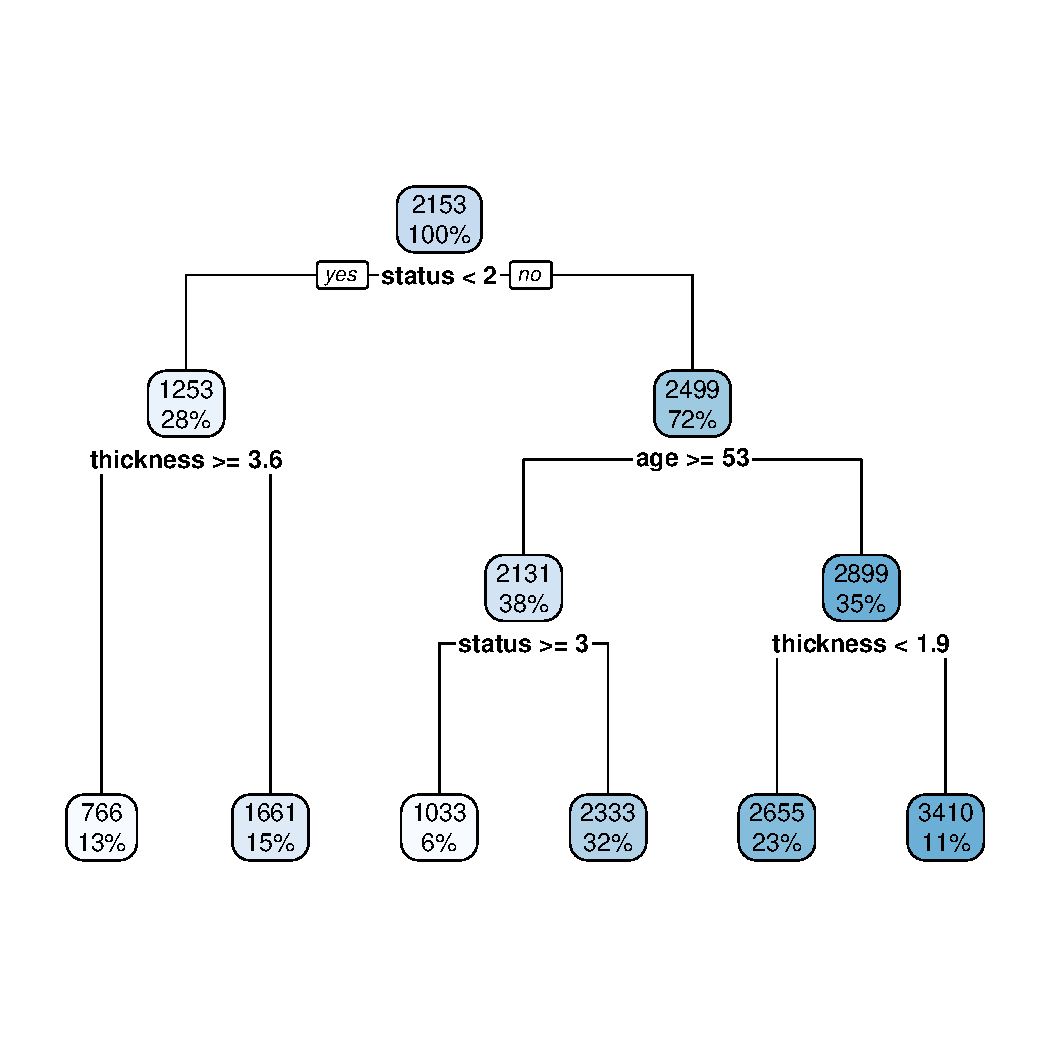
\includegraphics[width = 0.5\textwidth]{rpart_tree.pdf}
\end{figure} 

\end{frame} 



\begin{frame}
\frametitle{Look at learned model}
\vspace{2mm}
\begin{figure}
    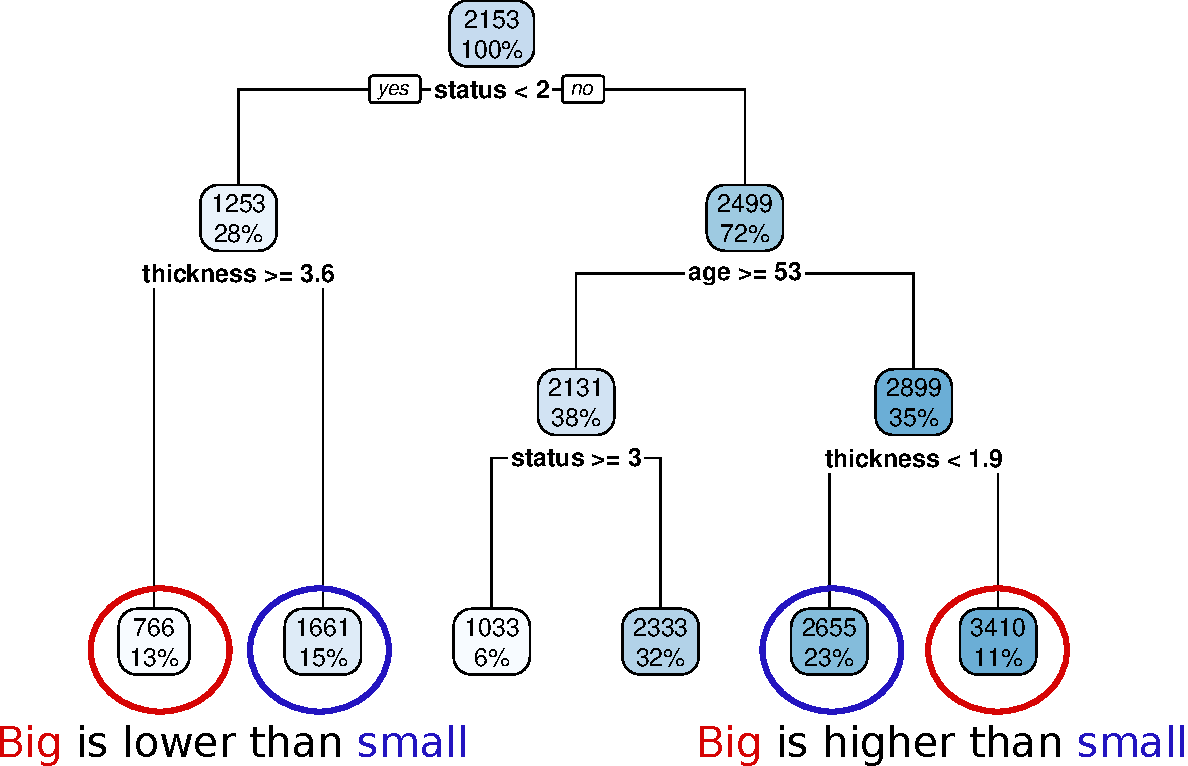
\includegraphics[width = 0.6\textwidth]{rpart_annotate.pdf}
\end{figure} 

\end{frame} 




\begin{frame}
\frametitle{What is machine learning?}
Supervised learning.

Classification or regression.
\begin{figure}
    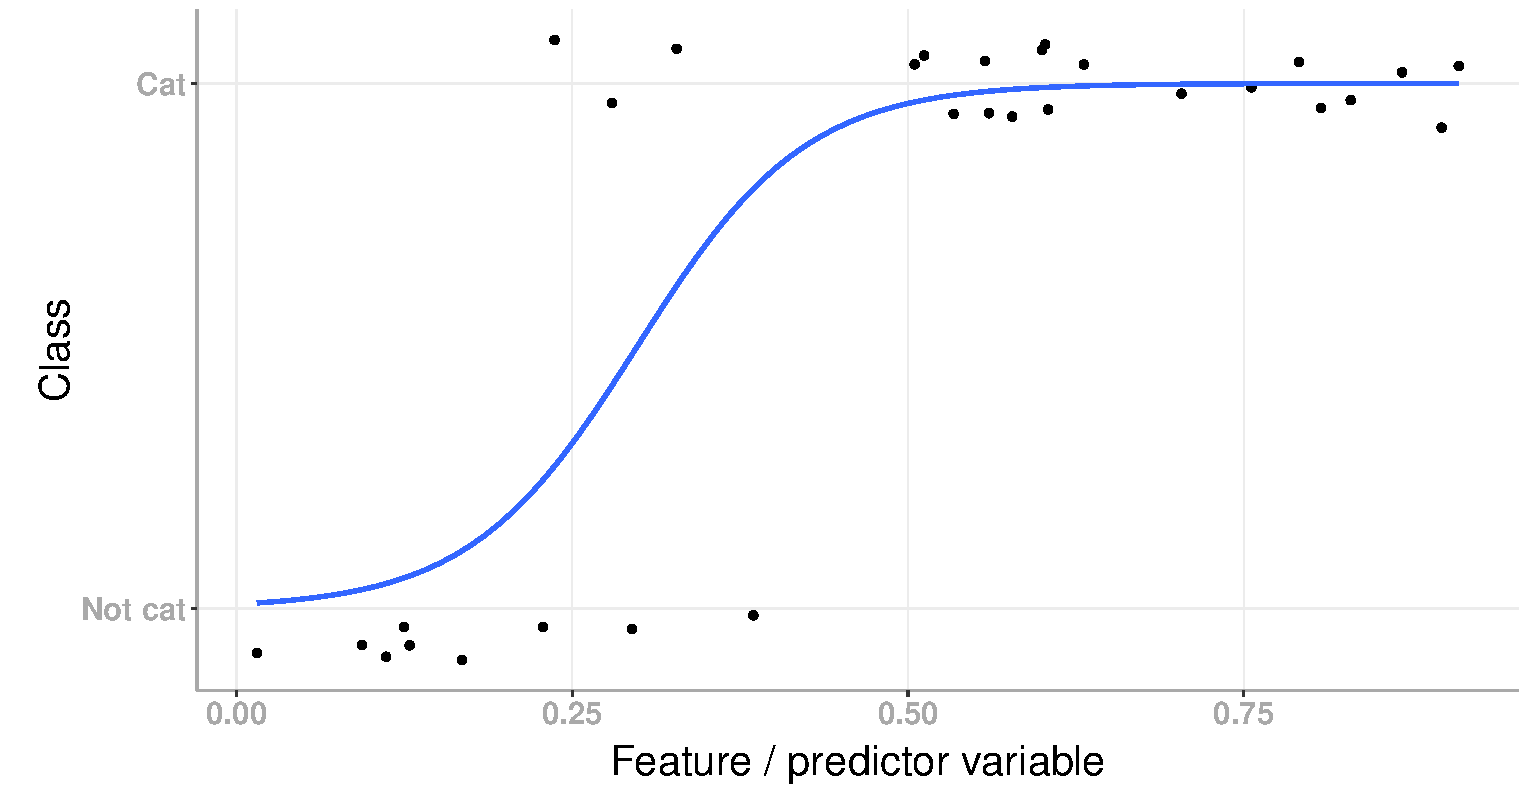
\includegraphics[width = 0.5\textwidth]{classification}%
    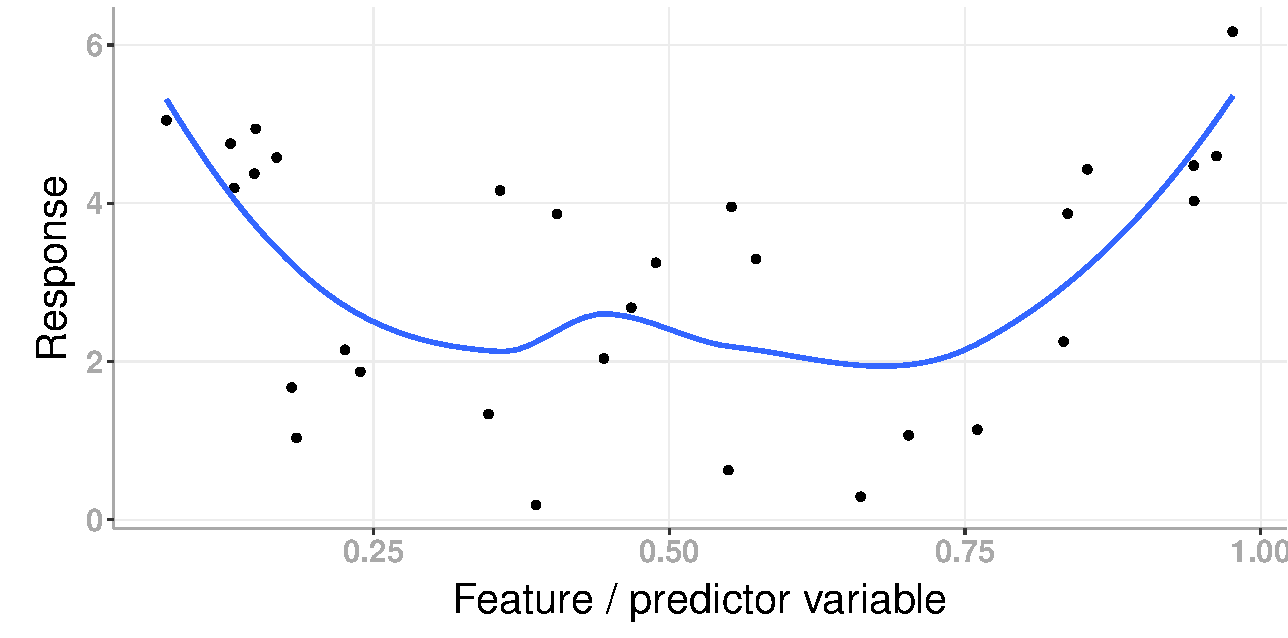
\includegraphics[width = 0.5\textwidth]{regression}
\end{figure} 

\end{frame} 


\begin{frame}
\frametitle{Caret package}
\begin{itemize}
\item https://topepo.github.io/caret/model-training-and-tuning.html
\item Unified interface to hundreds of models
\item Supervised learning
\item Full ML workflow
\item Excellent documentation
\end{itemize}

\end{frame} 


\begin{frame}
\frametitle{What is machine learning?}
Other tasks:
\begin{itemize}
\item Reinforcement learning
\begin{itemize}
\item Make your own data.
\end{itemize}
\item Unsupervised learning
\begin{itemize}
\item Clustering.
\end{itemize}
\end{itemize}
\end{frame} 











\begin{frame}[fragile]
\frametitle{What is ML good at? Predicting new data.}
\renewcommand{\FancyVerbFormatLine}[1]{%
   \ifnum\value{FancyVerbLine}=8\color{cyan}#1%
   \else #1\fi}
\begin{Verbatim}
tr <- trainControl(
        method = 'LGOCV',
        number = 1)

m1 <- train(time ~ ., 
            data = melanoma,
            method = 'rpart2',
            trControl = tr)

\end{Verbatim}

\end{frame} 






\begin{frame}[fragile]
\frametitle{What is ML good at?}
\renewcommand{\FancyVerbFormatLine}[1]{%
   \ifnum\value{FancyVerbLine}=7\color{cyan}#1%
   \else #1\fi}
\begin{Verbatim}
tr <- trainControl(
        method = 'LGOCV',
        number = 1)

m2 <- train(time ~ ., 
            data = melanoma,
            method = 'lm',
            trControl = tr)

\end{Verbatim}

\end{frame} 






\begin{frame}[fragile]
\frametitle{What is ML bad at?}
\renewcommand{\FancyVerbFormatLine}[1]{%
   \ifnum\value{FancyVerbLine}=1\color{cyan}#1%
   \else #1\fi}
\begin{Verbatim}
pl <- read.csv(
  file = 'https://raw.githubusercontent.com/timcdlucas/ml_workshop/master/planets.csv')

pl1 <- train(g ~ ., 
            data = pl,
            method = 'rf',
            trControl = tr)


\end{Verbatim}

\end{frame} 


\begin{frame}[fragile]
\frametitle{What is ML bad at?}
\renewcommand{\FancyVerbFormatLine}[1]{%
   \ifnum\value{FancyVerbLine}=1\color{cyan}#1%
   \else #1\fi}
\begin{Verbatim}
pl <- read.csv(
  file = 'https://raw.githubusercontent.com/timcdlucas/ml_workshop/master/planets.csv')

pl2 <- train(r ~ 0 + I(m1 * m2 / d ^ 2), 
            data = pl,
            method = 'lm',
            trControl = tr)

\end{Verbatim}

\end{frame} 





\begin{frame}[fragile]
\frametitle{Basic ML workflow}
\begin{Verbatim}
tr2 <- trainControl(
        method = 'repeatedcv',
        repeats = 3,
        number = 5)

m1 <- train(time ~ ., 
            data = melanoma,
            method = 'rpart2',
            tuneLength = 5,
            metric = 'MAE',
            trControl = tr2)

\end{Verbatim}

\end{frame} 




\begin{frame}
\frametitle{Maxdepth hyperparameter/tuning parameter}
\vspace{-4mm}
\begin{figure}
    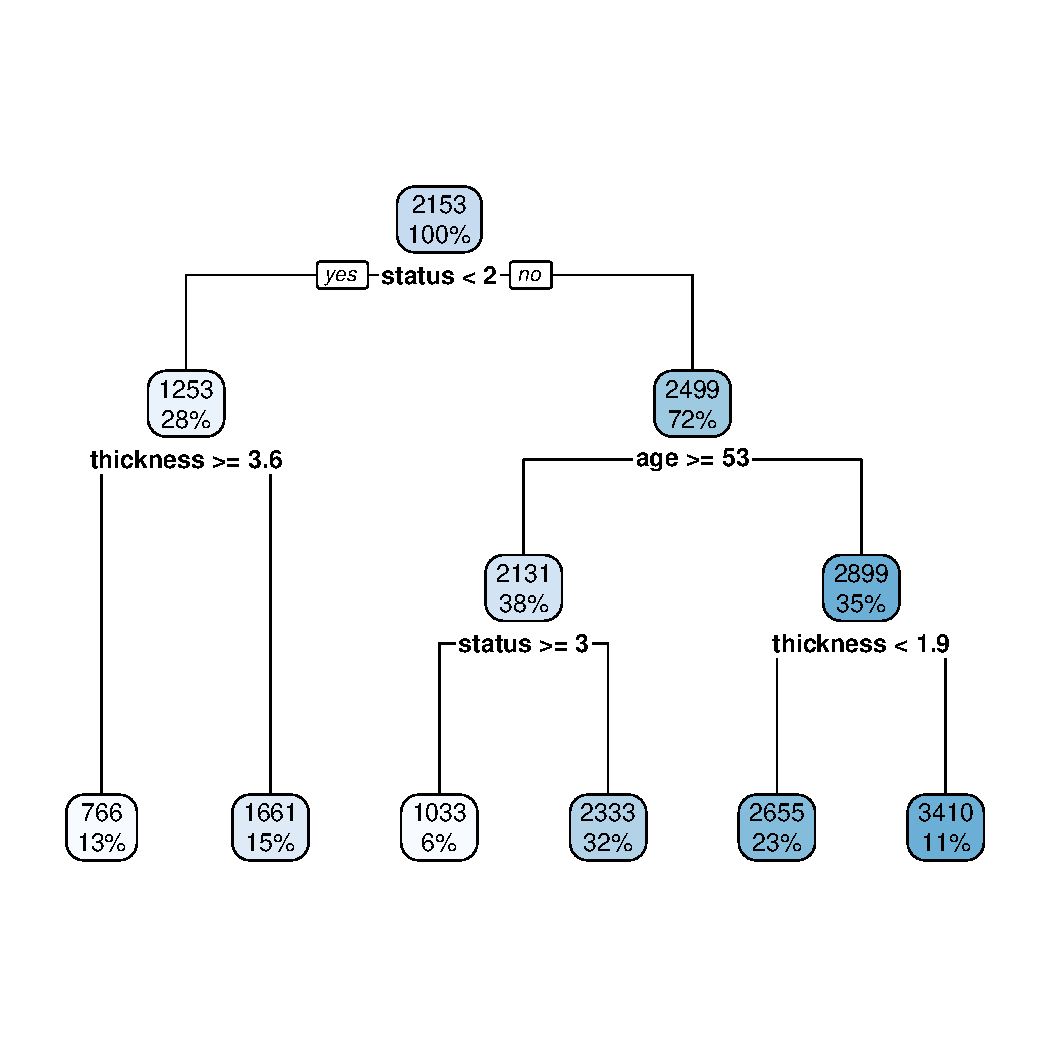
\includegraphics[width = 0.5\textwidth]{rpart_tree.pdf}
\end{figure} 

\end{frame} 







\begin{frame}[fragile]
\frametitle{Overfitting}
\renewcommand{\FancyVerbFormatLine}[1]{%
   \ifnum\value{FancyVerbLine}=7\color{cyan}#1%
   \else #1\fi}
\begin{Verbatim}
tr <- trainControl(
        method = 'LGOCV',
        number = 1)

m2 <- train(time ~ . + age^6, 
            data = melanoma,
            method = 'lm',
            trControl = tr)

\end{Verbatim}

\end{frame} 

\begin{frame}
\frametitle{Hyperparameters}
\begin{itemize}
\item Number of PCA coordinates
\item Cut-offs for variable selection
\item $x + x^2 + x^3 + x^4 + ...$
\end{itemize}
\end{frame} 

\begin{frame}
\frametitle{Hyperparameters}
\begin{figure}
 \animategraphics[loop,autoplay, width = 0.7\textwidth]{1}{scale-}{0}{2}
\end{figure} 
\end{frame} 



\begin{frame}
\frametitle{Cross-validation}
\begin{figure}
 \animategraphics[loop,autoplay, width = 0.6\textwidth]{1}{frame-}{0}{2}
\end{figure} 
\end{frame} 












\begin{frame}
\frametitle{No free lunch}
No such thing as a universal, `best' machine learning model.
\end{frame} 








\begin{frame}
\frametitle{What does caret do?}
\begin{figure}
    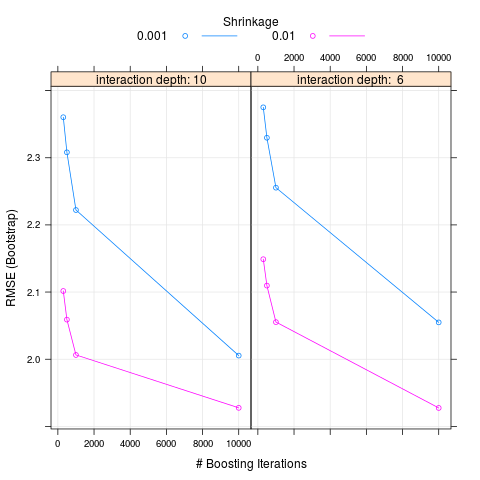
\includegraphics[height = 0.8\textheight]{gbm2opt}
\end{figure} 
\end{frame} 






\begin{frame}[fragile]
\frametitle{Training a model}
\begin{Verbatim}

m1 <- train(Species ~ ., 
            iris,
            method = `gbm')

\end{Verbatim}

\begin{figure}
    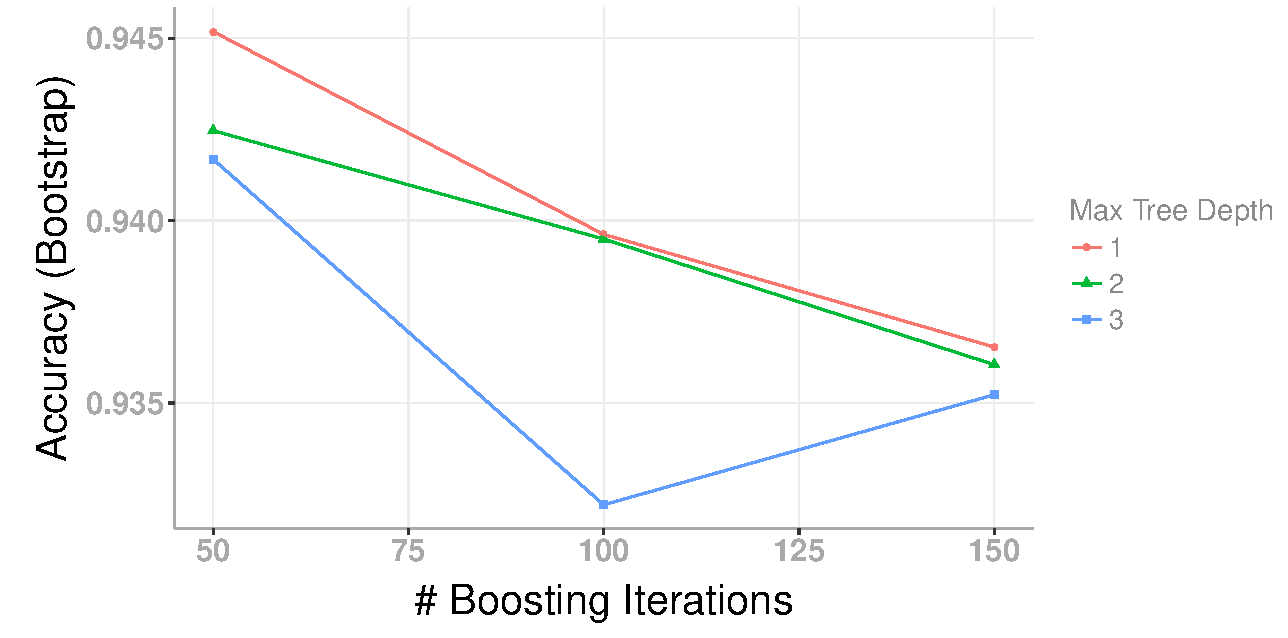
\includegraphics[height = 0.5\textheight]{train_gbm}
\end{figure} 
\end{frame} 


\begin{frame}[fragile]
\frametitle{Training a different model}
\renewcommand{\FancyVerbFormatLine}[1]{%
   \ifnum\value{FancyVerbLine}=3\color{cyan}#1%
   \else #1\fi}

\begin{Verbatim}
m2 <- train(Species ~ ., 
            iris,
            method = `nnet')
\end{Verbatim}

\begin{figure}
    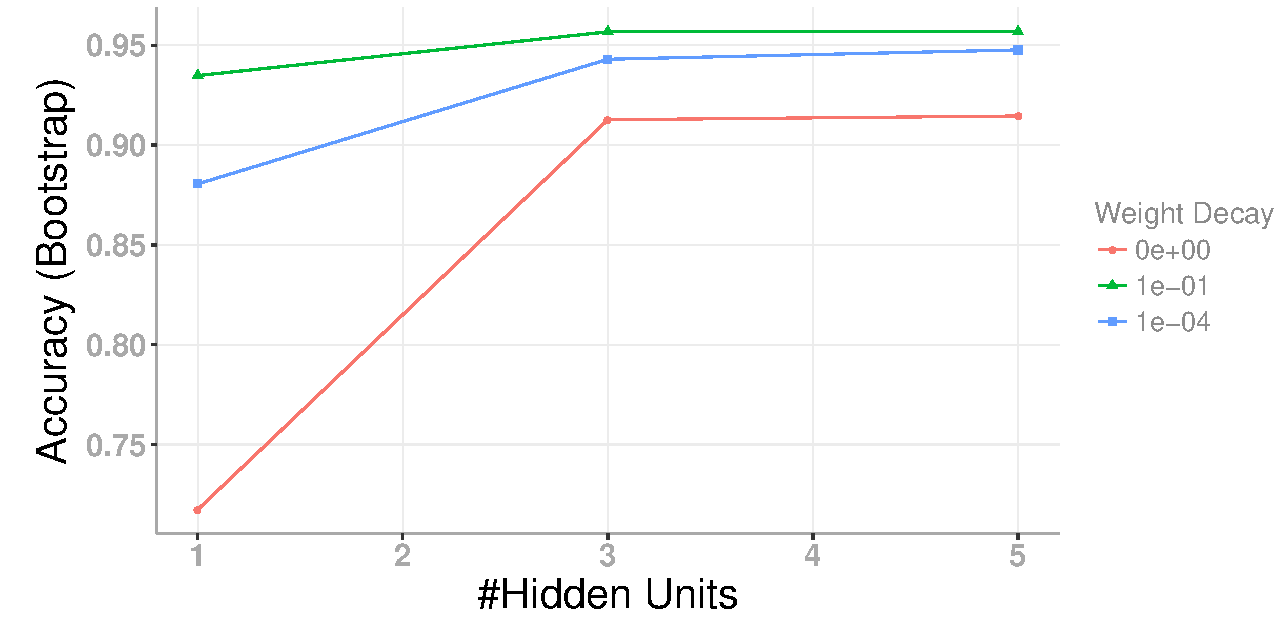
\includegraphics[height = 0.5\textheight]{train_nnet}
\end{figure} 
\end{frame} 




\begin{frame}[fragile]
\frametitle{Controlling Crossvalidation}
\renewcommand{\FancyVerbFormatLine}[1]{%
   \ifnum\value{FancyVerbLine}=1\color{cyan}#1%
   \else #1\fi}

\begin{Verbatim}
tr <- trainControl(method = `cv', number = 5)

m3 <- train(Species ~ ., 
            iris,
            trControl = tr,
            method = `nnet')
\end{Verbatim}

\end{frame} 



\begin{frame}[fragile]
\frametitle{Try more hyperparameter values}
\renewcommand{\FancyVerbFormatLine}[1]{%
   \ifnum\value{FancyVerbLine}=3\color{cyan}#1%
   \else #1\fi}

\begin{Verbatim}
m4 <- train(Species ~ ., 
            iris,
            tuneLength = 10,
            method = `nnet')
\end{Verbatim}

\begin{figure}
    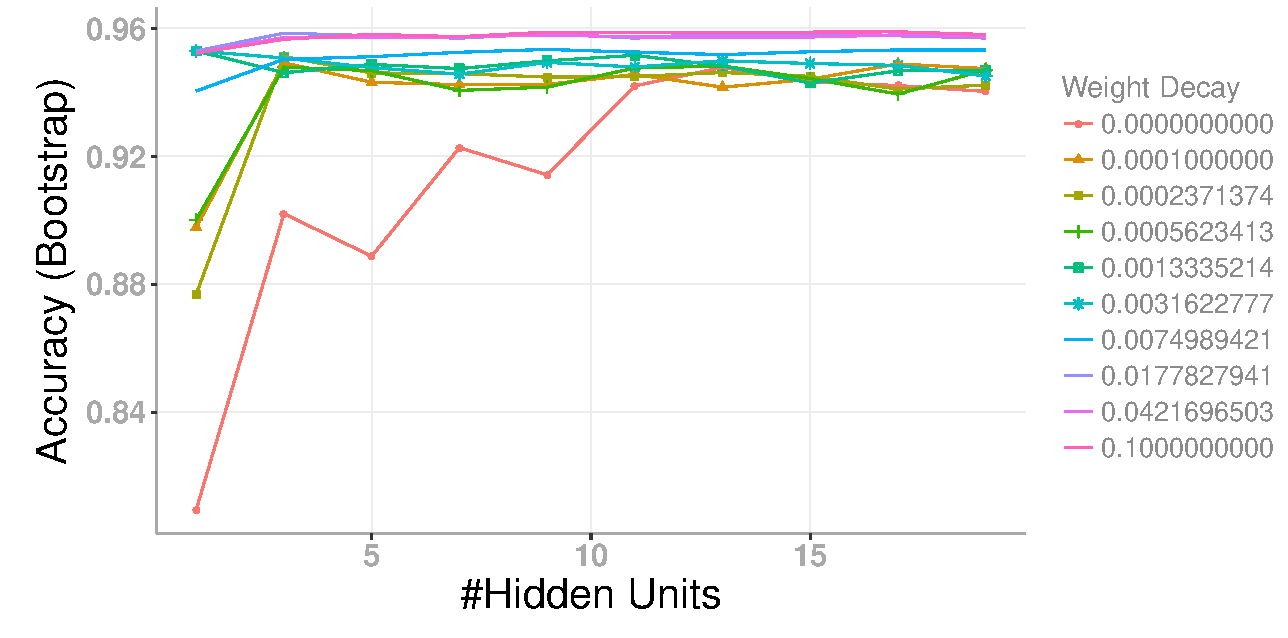
\includegraphics[height = 0.5\textheight]{train_nnet_tuneLength}
\end{figure} 
\end{frame} 





\begin{frame}[fragile]
\frametitle{Use chosen hyperparameter values}
\renewcommand{\FancyVerbFormatLine}[1]{%
   \ifnum\value{FancyVerbLine}=3\color{cyan}#1%
   \else%
   \ifnum\value{FancyVerbLine}=4\color{cyan}#1%
   \else #1\fi\fi}

\begin{Verbatim}
m5 <- train(Species ~ ., 
            iris,
            tuneGrid = expand.grid(size=c(1,5,10,20), 
                                   decay=seq(0,0.1,0.01)),
            method = `nnet')
\end{Verbatim}

\begin{figure}
    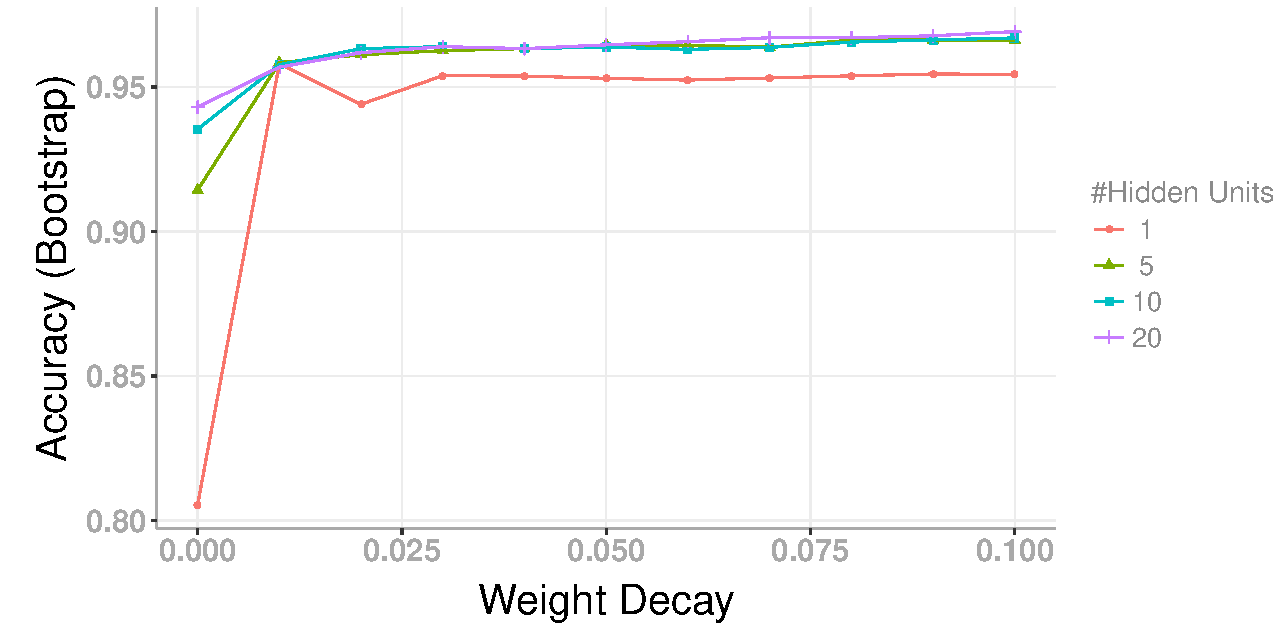
\includegraphics[height = 0.5\textheight]{train_nnet_tuneGrid}
\end{figure} 
\end{frame} 









\begin{frame}
\frametitle{Other packages}
\begin{itemize}
\item mlr
\item mlr3
\item tidymodels
\end{itemize}

\end{frame} 


    
\begin{frame}

\frametitle{Please ask me some questions}

\vspace{5mm}


\vspace{4mm}


\includegraphics[height=7pt]{Ar_Icon_Contact.pdf} tlucas{\footnotesize{@}}ic.ac.uk


\includegraphics[height=7pt]{Twitter_logo_blue-small.png} {\footnotesize{@}}statsforbios

\vspace{2cm}
\hfill % pushes logo the right
\includegraphics[width=5cm]{../../ceh_logo.png}

\end{frame}


%thanks


 
\end{document}


